\chapter{Результаты работы программы}

Внутри программы реализовано меню с выбором нужного задания, это мы можем увидеть на рисунке \ref{fig:tasks}

\begin{figure}
	\centering
	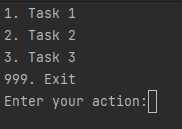
\includegraphics{inc/1}
	\caption{Меню выбора задания}
	\label{fig:tasks}
\end{figure}

\section{Задание 1}

На рисунке \ref{fig:1actions} мы можем видеть меню выбора действия

\begin{figure}
	\centering
	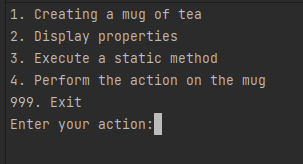
\includegraphics{inc/2}
	\caption{Меню выбора действия}
	\label{fig:1actions}
\end{figure}
